% !TeX root = ../main.tex

\chapter{相关技术基础}
本文工作开展在基于深度学习的神经辐射场之上,通过结合可微渲染实现了数字资产解耦管线,
致力于无缝对接传统渲染管线并解决其中的耦合问题。本章将介绍本文研究所必要的深度学习基础、
可微渲染理论基础、传统渲染管线介绍以及神经辐射场理论基础。

\section{深度学习基础}
【这里应该加点引言之类的】
\subsection{基于坐标的多层感知机}
多层感知机(Multilayer Perceptron, MLP)作为深度学习的基础模型,由感知机推广而来,
本质是一种前馈神经网络。MLP由多个神经元层组成,每个神经元的结构如图~\ref{fig:neuron}所示,其接收多个输入值,
并按照自身权重进行加权求和,接着,使用激活函数对其进行非线性变换,并将变换后的值传递给下一层神经元。

\begin{figure}[htb]
  \centering
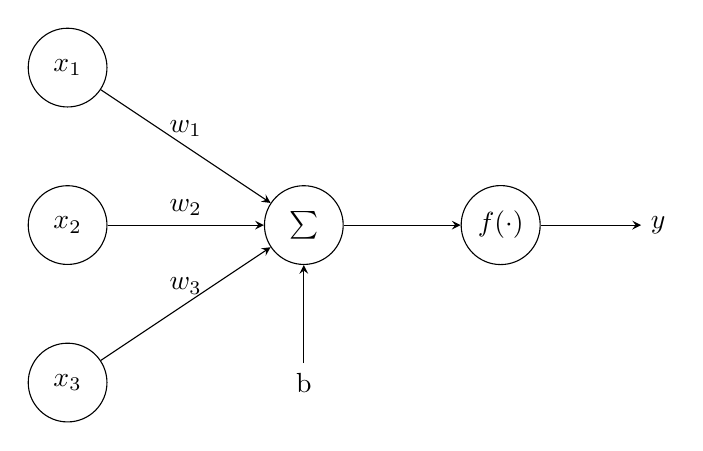
\begin{tikzpicture}[->,>=stealth, node distance=1.5cm, auto]
  % 定义输入节点
  \node[circle, draw, minimum size=1cm] (x1) at (0, 2) {$x_1$};
  \node[circle, draw, minimum size=1cm] (x2) at (0, 0) {$x_2$};
  \node[circle, draw, minimum size=1cm] (x3) at (0, -2) {$x_3$};

  % 定义偏置节点
  \node (bias) at (3, -2) {$\mathrm{b}$};

  % 定义神经元节点,内部写上激活函数(如 f(·))
  \node[circle, draw, minimum size=1cm] (sum) at (3, 0) {$\sum$};

  % 从输入节点到神经元的连线,并标注权重
  \draw (x1) -- node[midway, above] {$w_1$} (sum);
  \draw (x2) -- node[midway, above] {$w_2$} (sum);
  \draw (x3) -- node[midway, above] {$w_3$} (sum);
  % 从偏置节点到神经元的连线,标注偏置项
  \draw (bias) -- node[midway, below] {}(sum);

  % 定义神经元节点,内部写上激活函数(如 f(·))
  \node[circle, draw, minimum size=1cm] (activate) at (5.5, 0) {$f(\cdot)$};

  \node (y) at (7.5, 0) {$y$};

  \draw (sum) -- node[midway, below] {}(activate);
  \draw (activate) -- node[midway, below] {}(y);
\end{tikzpicture}
\caption{神经元的结构示意图}
\label{fig:neuron}
\end{figure}

多层感知机通过神经元从输入数据中学习到合适的参数权重和偏置项,利用激活函数将线性关系转化为非线性信号,
使得网络能够准确地完成各种分类或回归预测等方面的任务。这些信号从输入层通过一系列的隐藏层最终输出到输出层,
各层之间是完全连接的,具体如图~\ref{fig:mlp}所示:

\begin{figure}[htb]
  \centering
  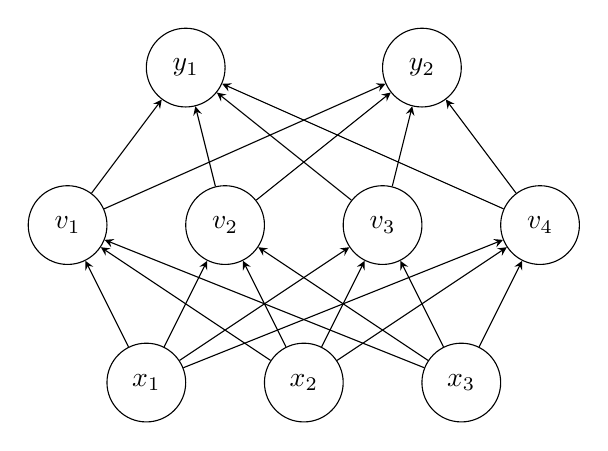
\begin{tikzpicture}[>=stealth, auto]

    % 定义公共变量
    \def\xspacing{2}      % 输入层和隐藏层的水平间距
    \def\layersep{2}       % 垂直层间距
    
    % 定义输出层特有的水平间距(可以调大该值)
    \def\outputxspacing{3} % 输出层水平间距
  
    % 输入层:3个节点
    \foreach \i in {1,...,3} {
      \pgfmathsetmacro{\xpos}{(\i-2)*\xspacing};
      \node[circle, draw, minimum size=1cm] (x\i) at (\xpos, 0) {$x_{\i}$};
    }
  
    % 隐藏层:4个节点
    \foreach \i in {1,...,4} {
      \pgfmathsetmacro{\xpos}{(\i-2.5)*\xspacing};
      \node[circle, draw, minimum size=1cm] (v\i) at (\xpos, \layersep) {$v_{\i}$};
    }
  
    % 输出层:2个节点,使用新的水平间距
    \foreach \i in {1,...,2} {
      \pgfmathsetmacro{\xpos}{(\i-1.5)*\outputxspacing};
      \node[circle, draw, minimum size=1cm] (y\i) at (\xpos, 2*\layersep) {$y_{\i}$};
    }
  
    % 连接输入层到隐藏层(全连接)
    \foreach \i in {1,...,3} {
      \foreach \j in {1,...,4} {
        \draw[->] (x\i) -- (v\j);
      }
    }
    
    % 连接隐藏层到输出层(全连接)
    \foreach \i in {1,...,4} {
      \foreach \j in {1,...,2} {
        \draw[->] (v\i) -- (y\j);
      }
    }
  
  \end{tikzpicture}
\caption{多层感知机的结构示意图}
\label{fig:mlp}
\end{figure}
根据通用近似定理\cite{Hornik_1989},只要给予网络足够多的神经元,MLP即可以任意精度逼近紧致集上的连续函数,
这一理论奠定了MLP作为函数逼近器的数学基础。然而,传统MLP多用于处理向量化特征(如图像分类中的扁平化像素),
其输入空间通常缺乏明确的几何语义。基于坐标的多层感知机(Coordinate-based MLPs)则突破了这一局限,
通过将空间坐标直接作为网络输入,并引入傅里叶坐标编码(Fourier Positional Encoding)
进行频域编码\cite{tancik2020fourier},
实现了对连续场函数的隐式建模,从而开创了三维几何与信号表示的新范式。

具体而言,直接使用原始坐标作为输入会导致 MLP 呈现明显的频谱偏差问题\cite{pmlr-v97-rahaman19a}。由于网络倾向于优先学习低频信号,
导致网络难以捕捉三维几何中的高频细节(如表面纹理、尖锐边缘等)。为此,研究者提出利用傅里叶坐标编码,
将 $d$ 维坐标 $\mathbf{x}\in\mathbb{R}^d$ 通过傅里叶基函数投影至高维空间。
傅里叶坐标编码可以由公式\eqref{eq:fourier_encoding}表示:
\begin{equation}
\gamma(\mathbf{x})=\left[\sin\left(2^0\pi \mathbf{x}\right),\cos\left(2^\pi \mathbf{x}\right),\ldots,\sin\left(2^{K-1}\pi \mathbf{x}\right),\cos\left(2^{K-1}\pi \mathbf{x}\right)\right]
\label{eq:fourier_encoding}
\end{equation}
其中 $K$ 为预设的频率层级,通过指数增长的频率项构造多尺度频带。
这种傅里叶坐标编码(Fourier Positional Encoding)使MLP能够显式访问不同频段的几何特征,
有效解决了频谱偏差问题。在神经辐射场(NeRF)等典型应用中,该技术被证明是实现高质量三维重建的关键因素。

\subsection{激活函数}

通过上文的介绍我们知道,在多层神经网络中,隐藏层仅能进行线性变换,因此仅由隐藏层组成的线性模型只
能拟合输入和输出之间的线性关系,无法处理非线性问题。为了增强模型的非线性表示能力,可以使用激活函数来加入非线性因素。
由于不同类型的激活函数对提高网络的非线性表示能力不同,所以针对不同的任务需要选择适合的激活函数。
当基于坐标的多层感知机使用ReLU等常见激活函数时,网络同样易于出现上文所述的频谱偏差问题。
ReLU激活函数的基本表达式如公式\eqref{eq:relu}所示:
\begin{equation}\label{eq:relu}
\text{ReLU}(x)=
\begin{cases}
x, & x>0,\\[1mm]
0, & x\leq 0.
\end{cases}
\end{equation}
它在 $x>0$ 时具有线性函数的特征,而在 $x\leq 0$ 时则恒定为0,这样可以使部分神经元的输出为0,
从而实现网络的稀疏性,缓解过拟合问题。此外,ReLU激活函数计算速度快,导数简单。
但是,这种单侧抑制机制虽能提升模型稀疏性,但其频谱响应呈现强烈的低频偏好:ReLU的导数在正区间为常数1,
负区间为0,其傅里叶变换能量集中于低频段。当应用于坐标输入时,ReLU的频谱偏差会抑制网络对高频几何细节
(如曲面曲率、纹理梯度)的捕捉,导致重建结果过度平滑。

为突破这一限制,Sitzmann等人\cite{sitzmann2020implicit}提出了SIREN(Sinusoidal Representation Networks),该网络创新性地采用正弦函数作为核心激活函数。
正弦激活函数可以由公式\eqref{eq:siren}表示:
\begin{equation}\label{eq:siren}
\phi_i(x_i)=\sin\Bigl(\omega_0\,W_i\,x_i+b_i\Bigr)
\end{equation}
其中 $\omega_0$ 为可学习的频率缩放因子。正弦激活函数通过周期性振荡特性,为神经网络引入频谱调制能力。
相较于ReLU,正弦函数的无限可微性及其导数的非零特性,使得网络可通过链式法则传递高频梯度信号,
避免频谱能量衰减。而权重矩阵 $W_i$ 与频率因子 $\omega_0$ 共同调节输入信号的频域分布,
使网络自适应平衡低频轮廓与高频细节的建模(如图\ref{fig:siren_compare}所示)。

\begin{figure}[htb]
  \centering
  % 这里可以控制图片宽度比例
  \includegraphics[width=0.6\linewidth]{Siren.png}
  \caption{激活函数对比\cite{sitzmann2020implicit}}
  \label{fig:siren_compare}
\end{figure}

实验\cite{sitzmann2020implicit}表明,采用正弦激活的MLP在3D形状重建任务中可将PSNR提升3-5 dB,
收敛速度加快5倍。这一突破性进展验证了激活函数频谱特性对隐式神经表示质量的决定性作用,
也为物理场仿真、微分方程求解等需高阶导数连续性的任务提供了新范式。

\subsection{损失函数}
【】【】这里还没写。

\subsection{自动编码器}
自动编码器(Autoencoder)作为深度学习中重要的无监督学习架构,其核心思想源于对生物感知系统中信息压缩与重建机制的仿生模拟。
该架构由对称的编码器(Encoder)与解码器(Decoder)网络构成,通过最小化输入数据与重建输出之间的差异,
迫使网络学习数据本质特征的紧凑表示。从数学角度来看,自动编码器可以看作是一种将高维数据转换为低维表示的工具:
编码器 $\mathcal{E}:\mathcal{X}\rightarrow\mathcal{Z}$ 将输入数据 $x\in\mathbb{R}^D$ 投影至 $z\in\mathbb{R}^d$ ,
解码器 $\mathcal{D}:\mathcal{Z}\rightarrow\mathcal{X}$则试图从潜在编码重构原始输入 $\hat{x}=\mathcal{D}\left(\mathcal{E}\left(x\right)\right)$,
其优化目标可以由公式\eqref{eq:ae_loss}给出:
\begin{equation}\label{eq:ae_loss}
\min_{\theta,\phi}E_{x\sim p_{\mathrm{dt}}}\Bigl[\bigl|x-\mathcal{D}_\phi\bigl(\mathcal{E}_\theta(x)\bigr)\bigr|^2\Bigr]
\end{equation}
其中$\theta$和$\phi$分别代表编码器与解码器的参数。这种方法不仅能在没有标注的数据中发现内在结构,而且在特征提取、
降维和去噪等应用中取得了很好的效果。早期的研究\cite{Hinton_2006}发现,当网络使用非线性激活函数并对低维空间进行一定限制时,
其能够有效地提取数据中的关键因素,比如在图像处理中自动识别边缘、纹理等重要视觉元素。

同时,自动编码器在处理复杂的光照估计与可微渲染问题时也有重要的作用。自动编码器的优势在于能够从高维数据中提取出最关键的特征,
并捕捉数据内在的低维结构。当我们面对真实世界的光照环境时(例如256\times256分辨率的环境贴图),
传统方法直接在原始像素空间进行优化会遇到三个问题:其一,像素数可能高达数百万,导致梯度下降等优化算法容易陷入局部最优;
其二,光照参数需要符合辐射度非负、能量守恒等物理规律,而仅仅依靠人工设计的正则项通常难以完全表达这些约束;
其三,实际光照中存在一些低维特性(如色温分布、主要光源的方向偏好),但要显式建立这些规律需要精确的先验知识。

因此,在可微渲染的任务里,自动编码器能够利用数据压缩的特性,通过编码器将高维环境贴图压缩到一个较低维的潜在空间,
构建出紧凑的光照参数表示,从而大大降低了优化问题的维度。同时,解码器将潜在向量映射回满足物理规律的光照配置,
确保优化过程中始终处于可行解范围内。这种“压缩-重建”机制实际上学习了一个数据驱动的光照投影操作,使得光照估计问题可以转化为在一个
平滑且低维的空间中进行高效搜索。例如,在同时优化物体材质和光照时,只需要调整潜在空间中的少量参数,就能获得物理上合理的光照重构,
而无需直接处理数百万维的像素数据。

\section{传统渲染管线}
本节介绍传统渲染管线的相关知识,为本文针对工作流进行光照分解补充相关背景知识。传统渲染管线中,
数字资产通常由网格体和多张纹理贴图组成,其中,网格体表达了数字资产的几何形状,纹理贴图和各类参数表达了数字资产表面不同的光学属性。
本节将介绍数字资产的制作和渲染过程,并解释数字资产与着色模型之间存在的耦合关系。

\subsection{渲染方程}


渲染方程(Rendering Equation)是计算机图形学中描述光与物体表面交互的基础方程之一。
由Kajiya等人于1986年提出\cite{Kajiya_1986},它为物体表面的光照计算提供了一个物理上合理的模型,
广泛应用于真实感渲染和计算机图像生成中。渲染方程通过描述光从场景中的光源到达表面并反射到观察者的过程,
计算表面点的辐射亮度(radiance)。具体计算过程如公式\eqref{eq:rendering_equation}:
\begin{equation}\label{eq:rendering_equation}
  L_o\left({\bf{x}},\omega_o\right)=\int_{\Omega}f_r\left({\bf{x}},\omega_i,\omega_o\right)\cdot L_i\left({\bf{x}},
  \omega_i\right)\left(\omega_i\cdot\mathbf{n}\right)\,\mathrm{d}\omega_i
\end{equation}
其中,$L_o\left({\bf{x}},\omega_o\right)$表示从表面点$\bf{x}$沿观察方向$\omega_o$看到的辐射亮度,
$L_i\left({\bf{x}},\omega_i\right)$是从入射方向$\omega_i$到达表面点$\bf{x}$的光源辐射亮度,
$f_r\left({\bf{x}},\omega_i,\omega_o\right)$是BRDF,
它决定了光线从入射方向$\omega_i$到反射方向$\omega_o$的散射方式,且依赖于表面的材质属性。
$\left(\omega_i\cdot\bf{n}\right)$表示入射光与表面法线$\bf{n}$的点积,代表表面与光源的接触程度,
而$\mathrm{d}\omega_i$是入射光方向的微小立体角元素。

渲染方程的核心思想是通过积分所有可能的光源对表面反射的贡献,计算出最终的观察光照。
其在实际应用中能够模拟多种光照现象,包括漫反射、镜面反射、折射以及其他复杂的光学效应。
然而,尽管渲染方程具有强大的表达能力,但其高计算成本使得在实时渲染中难以直接应用。
因此,许多基于渲染方程的模型需要进行简化或近似,以实现高效的图像生成。

\subsection{着色模型}

着色模型(Shading Model)是基于渲染方程的简化或近似,通常用于图形学中的实时渲染。其主要目标是通过简化光的反射过程,
使得渲染计算更加高效。通过引入一定的数学公式和参数设置,着色模型能够近似真实世界中的光照现象,
从而生成具有理想真实感或艺术效果的图像。
着色模型的核心是描述光线与物体表面相互作用的数学函数,输入通常包括入射光线、视角、表面法线以及材质属性
(如漫反射颜色、镜面反射强度、粗糙度等),输出则是某一点处的最终光照颜色或亮度。常见的着色模型包括:
\fourthtitle{1}基于物理的着色模型:这些模型遵循物理定律,精确描述光照现象,通常依赖于双向反射分布函数。
例如,Cook-Torrance模型[29] 通过微表面分布函数、几何遮蔽因子和Fresnel反射等参数,精确地模拟了金属和非金属表面的反射行为。基于物理的着色模型能够较为准确地模拟光的反射、折射和散射过程,生成更为真实的视觉效果。

(2)	经验性(非物理)着色模型:这类模型通常采用简化或经验公式来近似光照计算,
代表性的有Blinn-Phong模型和Lambertian模型。尽管它们并不完全遵循物理定律,
但通过经验参数(如光泽度、反射系数等)的调控,依然能够生成具有一定真实感的光照效果。
由于计算复杂度较低,经验性模型广泛应用于实时渲染或资源受限的场景。


